\chapter{Using the Linux desktop in CS}

Today we're going to explore some of the features of UNIX in a bit more depth, this time using the desktop PCs rather than your Raspberry Pi (we'll return to using that in the next lab). We'll explore some of the more advanced features of the command line and various useful tools that will help you understand how a typical UNIX system is organised. Almost everything that you learn today using Linux on the desktop machine is equally applicable to the Raspberry Pi, and vice versa. 

\section{Reading email at the console}

You're probably familiar with reading email using either a web-based interface, a graphical desktop application (such as Outlook, Thunderbird or OS X Mail) or using an app on a smartphone or tablet. Today you're going to do something slightly different, and configure a text-based mail client so that you can read your University email while at a console. The email client we're going to use is called Mutt, which is fairly simple to configure and straightforward to use (according to its author, Michael Elkins, ``All mail clients suck. This one just sucks less''). There are plenty of other similarly lean text-based \wikipedia{List_of_email_clients}{email clients}, and you may at some point want to check out Alpine as a sensible alternative to Mutt or for the historically-curious, Elm (if you want a \textit{really} hardcore console-mode experience of mail, look up \wikipedia{Mailx}{Mailx}).

First, let's confirm that Mutt is actually installed. Make sure the desktop PC is booted into Linux, and log in using your University username and password (not the username and password you used on the Pi). You should be greeted with a similar command prompt to the one you saw in the previous lab.

To see if Mutt is installed and is accessible to you, type

\begin{ttoutenv}
$ which mutt
\end{ttoutenv}

This should respond with \fname{/usr/bin/mutt}, telling us that the \fname{mutt} command has been put in the \fname{/usr/bin} directory on our system. Remember in the last sessions we looked at the contents of the \fname{/bin} directory that contained essential low-level commands such as \ttout{ls}? Well \fname{/usr/bin} contains commands that aren't quite as essential, but have been installed for the users' benefit (i.e. the system would boot/work without them, but it just wouldn't be very useful.)

List the contents of \fname{/usr/bin} by typing
\begin{ttoutenv}
$ ls /usr/bin
\end{ttoutenv}

and notice that here we're using \ttout{ls} to look at the contents of a directory other than the one we're currently in by passing the directory name as a parameter. A whole load of things should scroll past on the screen; most of them won't mean anything to you right now, but don't worry, we'll look at some of the important ones soon enough. Now that's a lot of stuff to look through, and depending on the size of your screen the command we're looking for may have scrolled off the top. So let's try to narrow our results down a bit. Type 
\begin{ttoutenv}
$ ls /usr/bin/m*
\end{ttoutenv}

and you should be given a much smaller list of things from the \fname{/usr/bin} directory; only those starting with the letter m. The asterisk symbol is interpreted as being a `wildcard' that stands for `anything of any length, including length zero', so the command you've just typed means `list the contents of the \fname{/usr/bin} directory, showing only files that start with the letter m and then are followed by zero or more other characters' (notice that the \ttout{man} command that you used in the last session is there amongst the results). 

You could narrow this down even further by typing \ttout{ls /usr/bin/mu*}, in which case you'll only get files from \fname{/usr/bin} that start with the letters mu. Note that if you leave off the asterisk from your command, you'll be asking for files that are called \textit{exactly} m or mu, which isn't what you want here.

So far we've been getting you to do a fair amount of typing, and now we have to admit that you've been typing a lot more than you actually need to (it's good practise though, so we're not feeling too guilty at this stage). The default Linux command line has a feature similar to autocomplete that you'll have seen on web forms and in graphical tools, that saves you typing full commands by suggesting possible alternatives. 

Type \ttout{ls /} but don't hit Enter, and instead press the Tab key twice. You'll be shown a list of sensible things that could follow what you've typed---in this case it's the list of directories that are in the system's root directory. Now type the letter u (so that the line you've typed so far should read \ttout{ls /u}) and hit Tab once. This time your command will be expanded automatically to \ttout{ls /usr/} since that's the only possible option. Press Tab twice now, and you'll get shown the contents of \fname{/usr/}. Type b, and press Tab to expand the command to \fname{/usr/bin/}, and then press Enter to execute the command.

The `autocomplete' function you're using here is more commonly called `tab complete' by UNIX users. If you press Tab once and there's only one possible option that would autocomplete what you've typed so far, then that option gets selected; if there are multiple possible things that could complete your command, then pressing Tab a second time shows you those, giving you the option to type another character or two to narrow down the list. Learning to use this will save you a lot of typing, because not only does it reduce the number of characters you type, it also helps you browse the options/files at the same time. 

Here are some other very useful command line tricks:

\begin{itemize}
\item You can use the up and down cursor keys to cycle back and forth through the list of commands you've typed previously.
\item The left and right cursors do what you expect, and move the insertion point back and forth. Pressing \ctrl{a} will move you to the start of the line, and \ctrl{e} to the end of the line (much faster than moving backwards and forwards character-by-character). 
\item \ctrl{c} aborts the current line, so if you've typed a line of gibberish, don't waste time deleting it one character at at time, just \ctrl{c} it!
\item Typing \ttout{history} lists all the commands you've typed in the past, useful if you've forgotten something.
\item Pressing \ctrl{r} allows you to retrieve a command from your history by typing part of the line (e.g. if you searched for `whi' now, it'll probably find the `which mutt' line you typed a while back). 
\item Pressing \ctrl{t} swaps the two characters before your cursor around. What, really? Yes: you'll be surprised how often you type characters in the wrong order! 
\end{itemize}

Back to configuring your email client. Before we use mutt, we need to point it at the incoming and outgoing email servers, and we'll do this by creating a configuration file.

\begin{diversion}{File extensions}
\label{diversion:file-extensions}
If you've mostly used Windows or OS X via a GUI, then you're probably used to files such as \fname{cheese.jpg}, where you would interpret \fname{cheese} as being the file \textit{name} and \textit{jpg} as being the file \textit{extension}. Some operating systems---notably Windows---have the notion of a \wikipedia{Filename_extension}{filename extension} of a particular number of characters built in; for example things ending with \fname{exe}, \fname{bat} or \fname{com} mean that they are executable files. In UNIX, a file extension is merely a convention that's not enforced or meaningful to the operating system. so although its common to give files a suffix that makes it easy for a human to guess what kind of file it is, Unix itself just treats these as part of the file name. In fact, you can have multiple `file extensions' in a name, to indicate a nesting of file types. In the previous lab the file \fname{quake3.tar.gz} is a `tar' archive that has been `gzipped', but the presence of the \fname{.tar} and \fname{.gz} parts are really just there to tell the user how to treat the file.
\end{diversion}

We've created a template file for you to get going with. Make sure you are in your home directory, then use the \ttout{curl} command as in the last lab session to fetch the template from \url{http://pod.cs.man.ac.uk/COMP101/mutt-template}. Remember, you're going to need to use a switch parameter to tell \ttout{curl} what it should call the file it's fetched: call it anything you like, but \fname{mutt-template} is a perfectly good name (if you're feeling uncomfortable about a file that doesn't have a file-extension, check out \ref{diversion:file-extensions} for more information). Let's look at the file to see what's in it. Type

\begin{ttoutenv}
$ less ./mutt-template
\end{ttoutenv}

and you should see the following written to the screen:
\begin{ttoutenv}
# Change the following six lines to match your University of Manchester account details
set imap_user = "mbnoodle"
set smtp_url = "smtp://mbnoodle@outgoing.manchester.ac.uk:587"
set from = "mister.noodle@stud.manchester.ac.uk"
set realname = "Mister Noodle"
set folder = "imaps://email.manchester.ac.uk:993"
set hostname = email.manchester.ac.uk

# Change the following line to a different editor you prefer.
set editor = "nano"
\end{ttoutenv}

The \ttout{less} command is used to display textual content from files and other sources (if you want to know why it has such an odd name, look at \ref{diversion:less}). 

\begin{note}
  Should they be using 'more' or 'less'
\end{note}

\begin{diversion}{Less is more}
As we've mentioned before, many of UNIX's commands are plays on words, puns, or jokes that seemed funny to the command's creator at the time. Though this gives UNIX a rich historical background, it does rather obscure the purpose of some commands. A prime example of this is the \texttt{less} command, used to page through text files that are too large to fit on a single screen without scrolling. 

Early versions of UNIX included a command called \texttt{more}, written by Daniel Halbert from University of California, Berkeley in 1978, which would display a page's worth of text before prompting the user to press the space bar in order to see \textit{more} of the file. A more sophisticated paging tool, called \texttt{less} on the jokey premis that `less is more' was written by Mark Nudelman in the mid 1980s, and has since replaced \texttt{more} in most Unix systems, including Linux. 
\end{diversion}

Don't worry too much about the details of this file for now. If you're already familiar with how IMAP and SMTP work together to provide your email service, then you'll be able to see how what the contents of this template mean; if you're not, don't worry, it'll all be explained in detail in the COMP18112 (Fundamentals of Distributed Systems) course in the second semester. For now, we just need to edit that file to contain your details rather than the fake ones in the template you've just downloaded. But lets play it safe: rather than editing the actual file you downloaded, just in case you make a mistake, let's first make a copy of the file in your home directory. Enter

\begin{ttoutenv}
$ cp mutt-template my-mutt-template
\end{ttoutenv}

Did you type all of that? If so, you've wasted several precious keypresses! You could have typed \ttout{cp mu}, and then pressed Tab to expand it to \ttout{cp mutt-template}, and then added on the \ttout{my-mutt-
template} bit yourself. It's a good habit to get into and will save you a lot of time over the next few years.

The basic form of the \ttout{cp} command takes two parameters, the first being the file you want to copy, and the second being the name of the file that will be created. Confirm that there is indeed a new file in your home directory using \ttout{ls}, and that its contents are what you expect using \ttout{more} (how would you find out what else the \ttout{cp} command could do?). 

To modify the file, you'll need to use a text editor. Type 
\begin{ttoutenv}
$ nano my-mutt-template
\end{ttoutenv}

to invoke the \ttout{nano} editor, and use it to change the text in square brackets the the correct values for you. Although fairly basic, the nano editor has all the features you'll need to make these changes, and helpfully shows you the various keyboard shortcuts to do particular things such as saving and quitting at the bottom of the screen (the caret symbol (\textasciicircum) is shorthand for `ctrl', so \textasciicircum X means '\ctrl{X}').

\begin{itemize}
\item $[$USERNAME$]$ should be replaced with your University username (which will be 8 characters, and will start with an m). Note you'll need to replace this on the lines with \ttout{imap\_user} and \ttout{smtp\_url}.
\item $[$FROM$]$ should be DUNNO!
\item $[$REALNAME$]$ is just your real name, in whatever way you want it to appear in outgoing emails.
\end{itemize}

When you've made the changes, write the file to your filestore and quit back to the command line. Then use \ttout{more} to confirm that the file now looks exactly as you want it to. 

Now, \ttout{mutt} expects the file containing its configuration information to have a particular name, and that's not \ttout{my-mutt-template}, so we'll need to do something about that. The UNIX \ttout{mv} command is used to rename files or directories (it's short for `move'), so use that to change the name of the file to \fname{.muttrc} by typing

\begin{ttoutenv}
$ mv my-mutt-template .muttrc
\end{ttoutenv}

Rather like \ttout{cp}, \ttout{mv} takes two parameters; but this time instead of making a copy of the file, \ttout{mv} just changes the name of the file given as the first parameter to that of the second. 

Type \ttout{ls} to confirm that the file name has changed as you'd expect. 

Oh. But it's gone! Actually, no, it's still there, but it's just hidden! There's a UNIX convention that files that start with a full-stop symbol don't appear when you type \ttout{ls} in its basic form, because these are normally configuration files that you don't need to see on a day to day basis (the `rc' part of the '.muttrc' name stands for 'resource configuration', another UNIX convention). So to see these files you'll need to add an extra switch parameter to \ttout{ls}. Use the \ttout{man} command to find out what this switch is, and then use the switch to confirm that the \fname{.muttrc} file does indeed exist. 

Using this switch on \ttout{ls} will reveal several other so-called `dotfiles' that have been lurking in your home directory all along. Use \ttout{more} to look at the contents of the one called \fname{.bash\_history} and it should become obvious how the \ttout{history} command, and the `reverse search' function you used earlier work.

If you're confident that you now have a file called \fname{.muttrc} containing the correct configuration, you can now type \ttout{mutt} to start the program. 

It should be reasonably clear how you use \ttout{mutt} to send and receive email; if you get stuck there are plenty of online tutorials to help you out. Send yourself a test email to make sure that everything is working, and when you're confident you've mastered the basics of sending and reading using this tool, drop back to the command line. One thing you should note is that \ttout{mutt} doesn't have its own editor for writing email, so will use \ttout{nano} to compose emails unless you change this to something else in the \fname{.muttrc} file. 

\section{Browsing the Web}

Although you will have experienced The Web so far as a highly graphical system, the technology that underpins it is for the most part text-based, and it is (just about!) possible to browse web pages using a console-mode application. It might seem like an odd thing to do, but there's an important point to be made here, so bear with us.

%and install the \ttout{lynx} package using \ttout{apt-get} (remembering you'll need also to use \ttout{sudo} to get root %privileges). 

%Once the package is installed

Try browsing the School's web pages using \ttout{lynx} by typing

\begin{ttoutenv}
$ lynx http://www.cs.manchester.ac.uk
\end{ttoutenv}

Rather like \ttout{mutt}, the \ttout{lynx} program has just about enough on-screen help for you to be able to browse around a little without any additional instructions from us.  You may find that when you follow some links, nothing very much appears to have happened; but scroll further down the page and you'll see the content that you're looking for.

You'll probably find using \ttout{lynx} an unsatisfying experience: tolerable, and probably okay in an emergency, but not how you'd ideally like to browse the web. And you might be wondering why we've even bothered to get you to try viewing the web through a text-only interface. Apart from the absence of images and videos etc., the main difference between using something like \ttout{lynx} and a regular browser such as Chrome, Firefox, Safari or Internet Explorer, is that you'll notice that web pages have been made into much more linear affairs than when they are rendered in a graphical environment. While you might expect to see the navigation links neatly arranged on the left or top of the page with the main content prominently displayed in the centre, seen through a purely textual interface it's all one big stream of stuff, and its very hard to distinguish between the navigation links and the main content. 

Now consider what the web `looks' like if you are visually impaired or blind and have to use use a screen-reader (a voice-synthesiser program that vocalises the text that's on-screen) to interact with your computer. Whereas a sighted person can easily cope with a two-dimensional layout that allows you to be aware of multiple things at the same time (i.e. you can be reading the main content of the page, but conscious of the fact that there's a navigation bar on the left for when you need it), if instead you are listening to a voice reading the contents of the page out to you, it's only possible to be hearing one thing at a time. And what's more, you have to remember what has been read out in the past in order to make sense of what you are hearing now; you can't just `flick back' a paragraph or two by moving your eyes, instead you have to instruct the screen reader to backtrack and re-read something. So the experience of using the web if you are visually impaired has some things in common to interacting with web-pages using \ttout{lynx}. 

You'll soon be designing your own web-based systems as part of the Group Project in this course unit; making them accessible to visually impaired readers something you should keep in mind. Try using \ttout{lynx} to browse some of your favourite websites, and you'll almost certainly find that the level of `accessibility' on the Web varies considerably!

\subsection{Pipes and Redirects}

One of the fundamental philosophies of Unix -- and one that is a sensible philosophy when you're building any computer system really -- is that the operating system is composed from lots of simple sub-systems, each of which performs one clearly defined task. To do something more complex than any of the individual tools allows you to do on its own, you are expected to combine components yourself. At the command line, Unix makes this quite simple, so let's give it a go. 

First, use lynx to look at the BBC's weather page at \url{http://www.bbc.co.uk/weather} and have a quick browse around to get familiar with what it looks like. Then quit lynx and get back to the command prompt before typing:

Type:
\begin{ttoutenv}
$ lynx -dump http://www.bbc.co.uk/weather
\end{ttoutenv}

Note the addition of the \ttout{-dump} parameter before the URL this time. Instead of running as an interactive browser, \ttout{lynx} should have just dumped the text that it would have displayed for that page to the console, and then quit. Now, most of the text of the page will have scrolled off the top of the screen, so let's use the \ttout{less} command to allow us to page through lynx's output in a more controlled manner. Type:

\begin{ttoutenv}
$ lynx -dump http://www.bbc.co.uk/weather | less
\end{ttoutenv}

Did you type all that? Hopefully not---remember you can use the up and down cursor keys to get previous commands back at the interactive prompt, and then just modify or extend them to save wearing out your fingers.

To explain what's happened here, you'll have to understand the concept of `standard in' and `standard out', which is a neat and extremely powerful idea that is fundamental to the way tools (and programmes generally) work in a Unix environment. 

Unless they are told otherwise, every Unix program has access to two ways of communicating with other parts of the operating system. The first, `standard in' allows a stream of data to be read by the program; the second, `standard out' gives the program a way of displaying textual responses. By default, when you execute things at the command prompt, Unix arranges for a program's standard in to be connected to whatever you type at the keyboard, and for its standard out to be connected to whatever display you're using at the time (this is a bit of an over simplification, but it'll do for now). It's quite easy to arrange for standard in and standard out to be connected up differently though, and that's what you've just done.

The vertical bar `\verb-|-' before \ttout{less} is called the `pipe' symbol, and it is used to join the output of one command to the input of another; so in this case we have connected the standard output from \ttout{lynx} directly to the standard input of \ttout{less} (when \ttout{less} is invoked without a filename argument, it expects to get its input from standard in). 

Instead of joining commands together, you can use the idea of manipulating standard in/out to create or consume files instead. Try:

\begin{ttoutenv}
$ lynx -dump http://www.bbc.co.uk/weather > weather.txt
\end{ttoutenv}

and then use \ttout{ls} to confirm that a file called \ttout{weather.txt} has been created, and use \ttout{less} to look at its contents (which should be just the text from the weather web-page we've been looking at already). Here the \verb-`>'- symbol redirects the standard out of the lynx command so that instead of going to the console display it gets put into a named file. 

To finish off this first contact with pipes and redirects, we'll use a new command called \ttout{grep} along with lynx to create a simple command of our own that tells you what the weather is like in Manchester (there are very few labs with windows onto the outside world in the Kilburn Building, so this may be more useful than you think!) 

Grep is a hugely powerful and useful utility, designed for searching through plain-text files. Learning to master grep will take more time than we have in this lab, since you'll have to understand the idea of \textit{regular expressions} to make full use of it (we'll come to those in \ref{sdjfosdifj}). For now, we'll use it in its very simplest form. Type:

\begin{ttoutenv}
$ grep BBC weather.txt
\end{ttoutenv}

and you should see a list of all the lines from \ttout{weather.txt} that contain the word `BBC'. Use \ttout{less} to have a look for other terms to `grep' for (you might want to try something like `Sunny' to give you a list of all the places where the weather is nice, for example). 

Rather like \ttout{less}, if grep isn't given the name of a file as its last command-line parameter (in this case we used \ttout{weather.txt}), it will operate on standard-input instead of grepping through a file (yes, it's quite okay to use grep as a verb from now, no one will look at you funny). Use this knowledge to join together lynx and grep so that the output is a single line describing the weather in Manchester right now. The output should look something like:

\begin{ttoutenv}
   [33]Manchester 22°C 72°F
\end{ttoutenv}

As a final flourish, let's create a new a way of accessing this new `weather in manchester' tool that you've created. Type:

\begin{ttoutenv}
$ alias mankyweather="[YOUR COMMAND GOES HERE]"
\end{ttoutenv}

replacing [YOUR COMMAND GOES HERE] with the full command line you created to display the Manchester weather. Then try typing

\begin{ttoutenv}
$ mankyweather
\end{ttoutenv}

to see the result. Okay, so this probably won't replace your favourite weather webpage or app, but its early days yet! 


\section{X Windows and Gnome} 

Next you're going to start up one of Linux's many graphical user interfaces. Type:

\begin{ttoutenv}
$ startx
\end{ttoutenv}

You'll see a chunk of text scroll up the screen briefly before being presented with something that looks like the screenshot in Figure \ref{figure:gnome-desktop}.

\begin{figure}[t]
\centerline{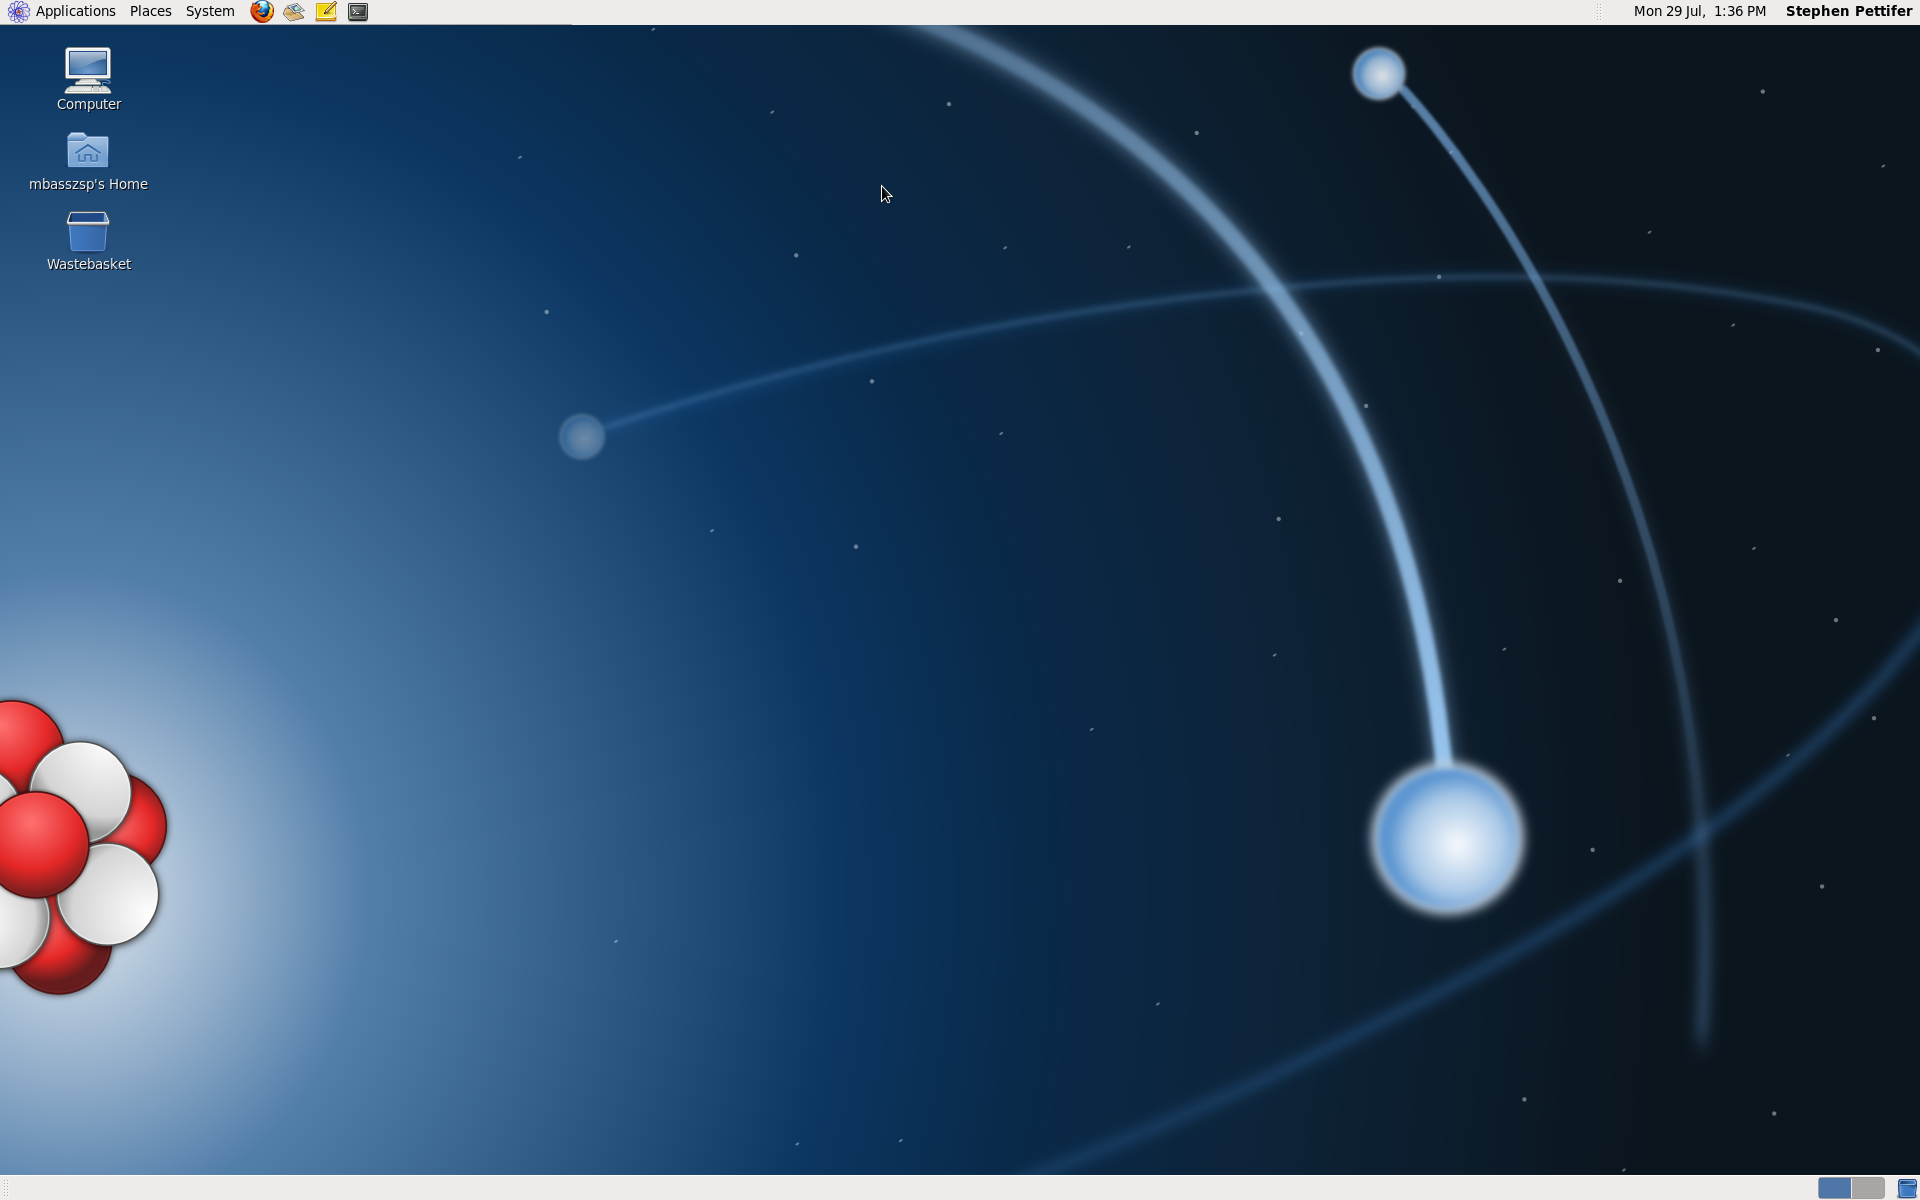
\includegraphics[width=16cm]{images/gnome-desktop}}
\caption{Scientific Linux's default graphical user interface and window manager, Gnome 2. \protect\circled{1} the top panel contains a menu of applications and system controls, as well as shortcuts to some frequently-used tools. You can easily configure the shortcuts to include your favourite things. \protect\circled{2} a graphical file-browser called `Nautilus' gives you graphical access to your files much like Explorer on Windows or Finder on OSX. \protect\circled{3} Clicking on your name shows the `log out' option. \protect\circled{4} The `wastebasket' and virtual desktop controls}\label{figure:gnome-desktop}
\end{figure}

Take a few minutes to explore the graphical environment. Even if you've never used Linux before, you'll probably find the general principles of this environment quite familiar: there are icons on the desktop giving you access to the computer via a graphical file browser, and at the top of the screen a menu-bar allows you to start various applications and utilities. The full manual for this environment---which is called Gnome 2---is available online at \url{http://personal.us.es/rledesma/descargas/gnome2.6-user-guide.pdf}, but you'll probably be able to work out everything you need to get you going by poking around at the various buttons. Unlike the Raspberry Pi where you have complete control over the operating system via the \texttt{sudo} command, the lab machines are configured so that you can't do any long-term damage to the setup. Apart from accidentally deleting your own files (and right now you have nothing to accidentally delete!), there's nothing much you can do that will cause problems, so feel free to explore a bit. 

Find out how to:
\begin{enumerate}
\item Find two ways of starting the Firefox web-browser.
\item Work out how to change the desktop theme. 
\item Find Application Blahdeblah. \ref{thingyblobbs}
\item Something else, and when you're done with these
\item Figure out how to log out of the graphical environment.
\end{enumerate}

If you've completed step 5 you should now be back at the command prompt where you typed `startx' a little while back. Before returning to the graphical environment where you'll spend most of your time, it's important to understand how the graphical interface you've just been using works as part of the Unix operating system. 

If you remember back to the first Raspberry Pi lab, we pointed out that the \texttt{shell} that you're using to interpret commands is `just a program' that happens to interpret input from the user, execute commands, and display the results. The graphical environment you've just used is similar -- just a program (or actually, collection of programs) that runs on the operating system.

But what do we mean by `execute commands'? You've probably got the hang of the fact by now that most of the things that happen in Unix are just programs stored somewhere on the file system (remember, you found some of them in the \texttt{/usr/bin} directory on the Pi). When you press return at a shell prompt, the program that is the shell checks that what you've typed has a valid syntax, and then starts up a new \textit{process} in which that program executes. The process is mostly independent of the shell program that started it, gets on with doing whatever it was designed to do, and when it finishes it tells the shell that it's done, and the shell gives you another prompt for the next instruction. Something very similar happens when you run the \texttt{startx} command: the graphical environment starts executing, and when you select the `log out' option, it returns you back to the shell so you can issue another command. Notice that you haven't been `logged out' of the machine, but rather just out of the graphical environment. 

Now, if you're going to use the graphical environment as your primary interface (and, as the jobs we ask you to do get more complex, you're going to need to!), you may find it slightly annoying to have to log into a lab machine, start the graphical environment, log out of the graphical environment when you're done \textit{and then remember to also log out of the console environment before you leave (because if you don't do this, other people will have access to your account!)}. 

Type the following:

\begin{ttoutenv}
$ exec ls
\end{ttoutenv}

You should find that the \texttt{ls} command has done exactly what you normally would expect, but that instead of returning you to the command prompt, you've been unceremoniously logged out! Log back in again (sorry about that). 

The \texttt{exec} command changes the way in which the shell deals with whatever command follows it. Instead of starting a new process in which to run your command and waiting in the background for that command to complete, the shell gives up the process in which it itself is running, and hands it over to the command you've issued. So when that command finishes, there is no shell to come back to. And because in this case the shell was the first program that got run when you logged in, the Unix system logs you out since there's nothing else you can do. 

Experiment by running \texttt{exec startx} and then logging out of the graphical environment as you did a moment ago; this time you should find that you've automatically been logged out of the console too.

But although that's one step closer to what we want, there's still the issue of having to type \texttt{exec startx} every time you log in. Of course this isn't a huge deal (it's certainly not as annoying as accidentally leaving yourself logged in at a console), but we can do better than this. 

When you first run the bash shell, it looks for a file in your home directory called \texttt{.bash\_profile} and executes any commands it finds in there as though you'd typed them at the keyboard. Use the \texttt{ls -a} command to confirm that there's already a file in your home directory called \texttt{.bash\_profile}, and then use \texttt{less} to look at its contents.

It should look something like this:

\begin{ttoutenv}
# .bash_profile

# Get the aliases and functions
if [ -f ~/.bashrc ]; then
	. ~/.bashrc
fi

# User specific environment and startup programs

PATH=$PATH:$HOME/bin

export PATH
\end{ttoutenv}

though don't worry if there are slight differences. We'll come back to what these instructions mean a little later one. For now, fire up the \texttt{nano} editor, and use it to add a new line at the end of your \texttt{.bash\_profile} that reads 

\begin{ttoutenv}
exec startx
\end{ttoutenv}

Now log out (either type \texttt{logout} or press Ctrl+D), and log back in again. If all has gone to plan then you should see the graphical environment fire up automatically; and when you select `logout' from the menu, you should be returned to the Linux login prompt. 

Hurray!




\section{X Windows}

Let's take a step back now and look at what the \texttt{startx} command has actually done. Unlike operating systems such as OS X and Windows, Linux doesn't really `have' a graphical windowing environment `built in'; what you've seen just now is a series of programs that co-operate with one another to give create the familiar WIMP environment. 

\begin{figure}[htb]
  \begin{center}
    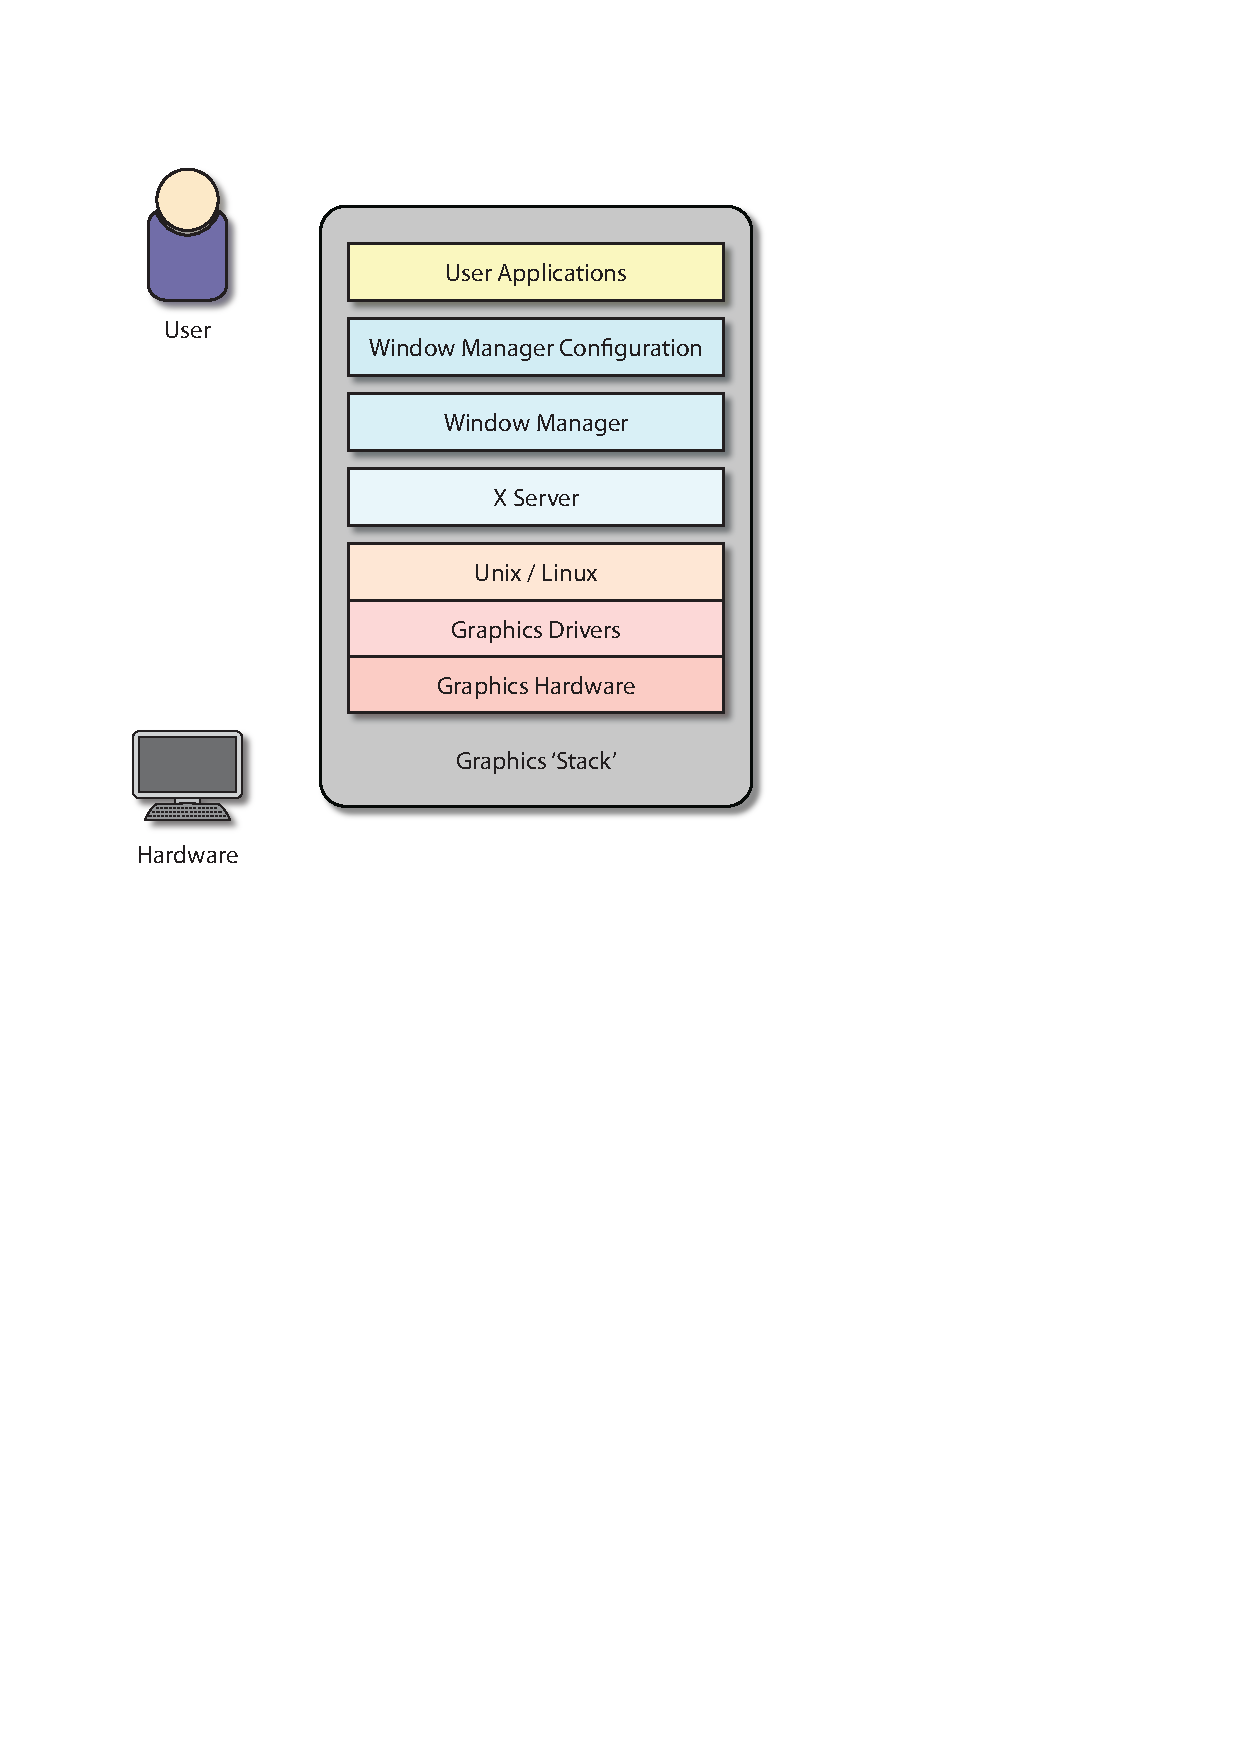
\includegraphics[width=12cm]{images/graphics-stack.pdf}
  \end{center}
\caption{The layered structure of Linux's graphical system, with software nearest to the underlying hardware at the bottom, and software closest to the user at the top.}
\label{figure:Xstructure}
\end{figure}


When you ran Quake and the snake game on the Pi in the previous lab, these programs took direct control of the graphics subsystem in order to display the game. The \texttt{startx} command runs a system called \wikipedia{X_Window_System}{X Windows}, which also communicates with the computer's graphics system, but on its own doesn't really do anything very exciting apart from allow other programs to then share the display. Along with X Windows, another system called a \wikipedia{Window_manager}{Window Manager} (in this case, called Gnome) was started, and this is what you see drawing the buttons and menus and window controls for the graphical user interface. We'll look at how X Windows really works in one of the forthcoming COMP101, and you'll explore the architecture of X Windows in a lot more detail in COMP18112 (Fundamentals of Distributed Systems) in the second semester. For now, it's enough to understand that there are two things going on here, first the X Windows system is running that allows stuff to be drawn to regions of the screen, and second the Window Manager which is doing all the WIMPy stuff like providing all the controls that allow windows to be moved and resized. 

One of the interesting effects of this architecture is that you can use different window managers on Linux, and can choose the one that best suits the way you work; some people like `rich' environments like Gnome, whereas others like `lean' cut-down window managers. 

To demonstrate this, use nano to create a file in your home directory called \texttt{.xinitrc}, and in that file put a single line that reads:

\begin{ttoutenv}
BLAAAAAAAH
\end{ttoutenv}


\begin{note}
Test out which other WMs are installed; can you kill X server from the keyboard?
\end{note}

%\printbibliography

\section{Terminal stuff}

Run some commands in an xterm, including mutt.

\section{Graphical Editors}



\section{Configuring Thunderbird}

\section{Exploring the CS UNIX environment -- which RPMs are installed}



